\section{Padrão Arquitectural - Dependency Injection}
\label{sec:dependency}

\begin{figure}[H]
    \centering
    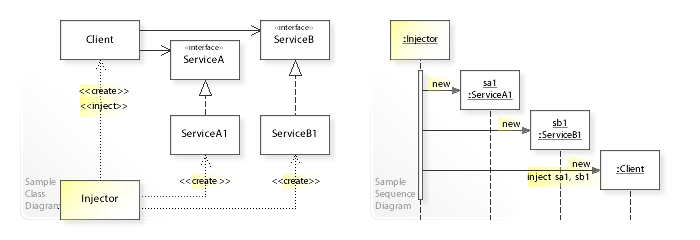
\includegraphics[scale=0.6]{images/dependency-injection.jpg}
    \caption{Dependency-injection.}
    \label{fig:dependency-injection}
\end{figure}

\hspace{3mm}O \textit{pattern} arquitectural \textit{dependency-injection} consiste numa técnica utilizada na construção de aplicações, onde um objecto declara as dependências de outro. 

Uma \textbf{dependência} representa-se como um objecto, sendo este usado por exemplo como uma funcionalidade/serviço de uma aplicação, por outro lado, objectos que usem outros (objectos/funcio-nalidades/serviços) são considerados \textbf{clientes}.

A expressão "\textit{dependency injection}"\ utilizada na nomeação deste \textit{pattern}, deve-se ao facto do objecto \textbf{Injector}, criar e injectar/passar as \textbf{dependências}/\textbf{serviços} ao objecto \textbf{Client} como argumento, para que este os possa utilizar. Tal como se pode verificar na figura \ref{fig:dependency-injection}, no diagrama de sequência, a criação por parte do \textbf{Injector} dos serviços, seguida da injecção dos mesmos no \textbf{Client}, também criado pela classe \textbf{injectora}.

Os principais objectivos deste \textit{pattern} arquitectural consiste na redução das dependências, bem como a separação das responsabilidades (criação e uso de objectos), com a finalidade de aumentar a fiabilidade e reutilização de código. Mas poder-se-á pensar o porquê da necessidade da separação destas responsabilidades. A razão consiste que o \textbf{Client} não deve criar os \textbf{objectos}/\textbf{serviços} através dos construtores destes, isto porque, no ponto de vista de evolução de código, se houver alterações à instanciação destas classes, vai ser necessário modificar o código do \textbf{Client}. 

A solução encontrada, como já foi referido anteriormente, foi a injecção dos \textbf{serviços}, de forma a "impedir"\ que o \textbf{Client} saiba como são construídos, sendo isto da responsabilidade do \textbf{Injector}. O \textbf{Client} não executa qualquer código do \textbf{Injector} (não dependendo do mesmo), apenas conhece as interfaces dos \textbf{serviços}, definindo-se nestas os métodos que o \textbf{Client} pode utilizar do respectivo \textbf{serviço}, tal como se pode verificar na figura \ref{fig:dependency-injection}.

Aparentemente, o \textit{dependency-injection} parece muito semelhante ao \textbf{Abstract Factory}, no entanto, a grande diferença consiste em não ser necessário instanciar no \textbf{Client} o \textbf{factory}/\textbf{injector}, para a criação dos \textbf{objectos}/\textbf{serviços}, reduzindo assim as dependências. Por outro lado, o \textit{dependency-injection} injecta/cria serviços, mas também pode apenas injectar serviços já existentes, sendo desta forma, diferente do \textbf{Abstract Factory}, que apenas cria objectos.

O \textit{dependency-injection}, pode ser aplicado de diferentes formas, sendo a diferença entre elas, a forma como se injecta os \textbf{objectos}/\textbf{serviços}. Apesar de existirem várias formas de aplicar o \textit{pattern}, apenas serão apresentadas as três mais importantes: \textit{constructor injection}, \textit{setter injection} e \textit{interface injection}. O \textit{constructor injection}, passa os \textbf{objectos}/\textbf{serviços}, pelo construtor do \textbf{Client}. O \textit{setter injection}, define um método na classe \textbf{Client}, para efectuar a passagem dos \textbf{objectos}/\textbf{serviços}. Por fim, \textit{interface injection}, bastante semelhante ao anterior, no entanto, a diferença consiste que neste caso, define-se uma interface, com o método para a passagem dos \textbf{objectos}/\textbf{serviços}, para "obrigar"\ o \textbf{Client} a defini-lo.

No entanto, o \textit{pattern}, não consegue ser perfeito, contendo algumas desvantagens, das quais, dificuldades de análise/leitura do código, por parte dos \textit{developers}, visto que, separa a criação do comportamento dos objectos. Do mesmo modo, devido ao facto de se mover a complexidade para fora das classes e passa-la para a interligação entre as mesmas torna-se mais complicada a sua gestão, entre outras desvantagens.

